\section{Planning and Execution with \rx}
\label{sec:arch}

\subsection{Introduction}
\label{sec:arch:intro}

A prime motivation behind the \rx architecture was to design a
controller which could bring automated planning closer to low-level
control of the vehicle while maintaining its reactivity. 

Traditionally planning has been deemed computationally expensive with
planner performance restricting robot reactivity
\cite{ghallab04,Dias:2003ua}. In control architectures where task
planning is embedded, planning consequently remains at an abstract
level with the assumption that it would otherwise impede system
reactiveness and that the environment can change at a faster rate than
the planner can plan for. In such a situation, the agent may thrash if
the internal state of the plan gets out of synch with the actual state
of the world. As a result the planning problem managed {\em in situ}
has traditionally remained fairly detached from low-level
control. Most adaptations at the lower-level reactive layers in
contrast are managed by specialized components (for example
\texttt{LAAS architecture} \cite{alami:1998p820,Ingrand07} and
\texttt{CLARATy} \cite{Nesnas:2003do}) that rely on different
representations for modeling local control behavior or worse do not
have any explicit formal agent behavior model. The consequent
different techniques for specifying each layer in the architecture
results in duplication of effort and a diffusion of knowledge leading
to significant design and integration issues \cite{DS1report}.
\texttt{IDEA} mitigated most of these issues by tightly integrating
planning and execution in a single representational and computational
framework with \kcomment{an} unified declarative model. Our approach
with \rx builds on this design methodology albeit in a substantially
systematic manner. The \rx architecture contributes to agent
architectures over and beyond \texttt{IDEA} in the following
\kcomment{significant} ways:

\begin{itemize}

\item \emph{Partitioning} the global planning problem into multiple
  decision loops, called {\em reactors}. Each reactor has its own
  scope both functionally (one for example focusing on the conversion
  of high level waypoints into low-level commands) and temporally as
  each reactor declares its planning look-ahead $\pi$ and expected
  latency $\lambda$ before being able to produce \kcomment{a} plan to
  the agent depending on where it is located in a reactor dependency
  graph such as shown in Fig. \ref{fig:agent}. A reactor closer to the
  hardware in the hierarchy, is expected to deliberate less and be
  highly responsive to observations from the world. This implies lower
  values of $\pi$ and $\lambda$ (see Section \ref{sec:arch:trex}
  below).

\item \emph{Coupling} a tighter integration between the planning
  process and world evolution to ensure that planning occurs
  \emph{during continuous} state update in the {\em same}
  \kcomment{plan} database used for planning. By doing so, the planner
  is better informed in its deliberation despite a larger latency than
  the changing world.
\end{itemize}

Systematic partitioned inference is a major contribution of
\rxe. However that is not the focus of this chapter with details
covered in \cite{py10, rajan12}. Coupled interaction between planning
and the world on the other hand, has a significant implication on how
planning can be integrated in such frameworks. In this chapter we show
how using the \eu planner can be coupled to our framework by first
linking concepts in temporal planning with the \rx framework. Note
that in the following treatise, we call the formal semantic framework
of \rx as the 'agent'. Reactors constitute an entity within this agent
and are standalone blocks of inference. The scope, detail and number
of reactors are application specific and outside the scope of this
chapter.

% on should integrate a
% planner in this framework in general and was applied to the europa
% framework specifically. We'll develop later how this requirement
% implies to see in-situ planning as two parallels processes that are
% tightly linked through the same plan structure. But before that we
% need to introduce at least the high leve lconcepts and ideas behind
% our architecture as a whole.

\subsection{Architectural concepts in \rx}
\label{sec:arch:trex}

The \rx architecture is structured around the notion of \eu {\em state
  variables} as the fundamental basis of interaction. Additionally it
comes with a well-defined ownership model associated with each such
state variable. In this framework each reactor is seen as a 'black
box' providing its own {\em internal} state variable which it is
responsible for in order to maintain its value at every instant of
time. Each such instance is represented by a {\em tick} with a fixed
duration; in our implementation of \rx on the Dorado AUV, we use a
tick of $1$ second. In order to identify its state a reactor can
subscribe to {\em external} state variables owned by other reactors,
for which it will receive new updates when the owner reactor generates
its {\em internal} state.

% \begin{figure}[!htbp]
%   \centering
%   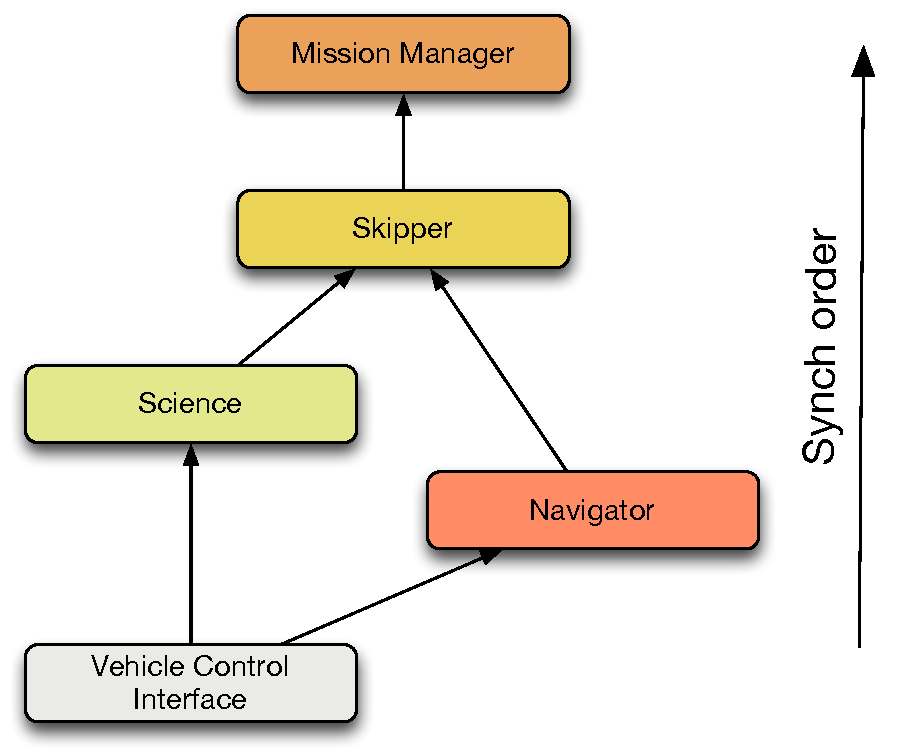
\includegraphics[scale=0.35]{figs/DAG-hierarchy}
%   \caption{\small An example of a \rx reactor hierarchy which is used
%     to determine a synchronization order for propagation of values in
%     \emph{external} state variables.}
%   \label{fig:reactor-DAG}
% \end{figure}
% \fcomment{I removed this figure as the next one is mucjh more
%   detailed and vehiculate the same idea}

As the execution frontier, $\tau$ advances, the \rx agent propagates
the current state information across all reactor state variables
through the {\em synchronization} process.  The sequencing of the
reactors synchronization is identified by traversing a reactor
dependency graph from the least dependent -- ones with no {\em
  external} state variables -- to the most, \ie which typically do not have
{\em internal} state variables. Fig. \ref{fig:agent} shows an example
of such a dependency graph implemented as a directed acyclic graph.

Conversely each reactor can request a future change on one of its {\em
  external} state variables which will be transformed as an {\em
  internal} goal to the owner reactor(s).  Such \emph{goal
  dispatching} is expected to produce a deliberation phase for the
receiving reactor which can cyclically in turn, produce a plan
impacting its {\em external} state variables' future that will
propagate down following the same mechanism.

In such a process, one challenge is to avoid being overwhelmed by
goals that may threaten the ability of a reactor to process and
integrate in its evolving partial plan. For that reason, each reactor
specifies the following two parameters that \kcomment{are} applied
towards the scope of the agent lifetime:

\begin{itemize}

\item $\lambda$ is the specified latency of this reactor, which is an
  indicator of the \emph{maximum expected time} for a reactor to
  produce a plan.\footnote{Note that while it is highly recommended to
    select a sound value, a failure to produce a plan within a chosen
    value for this parameter is not considered as a critical failure
    of the reactor.}

\item $\pi$ is the planning \emph{look-ahead} of the reactor. which is
  indicative of the number of ticks in the future this reactor is
  looking ahead during deliberation.

\end{itemize}

Using this information along with the dependency relation between
reactors, \rx defines the notion of execution latency of a state
variable as follow:

\begin{definition}
  The {\em execution latency} of a {\em state variable} $s$ which is
  internal to the reactor $r$ is the maximum expected delay before a
  goal on this state variable can be included in its plan and executed
  by the reactor $r$. It is defined recursively as: 
  \begin{equation*}
    \lambda_{exec}(s) = \lambda(r) + \max_{e \in exts(r)}
    \lambda_{exec}(e) 
  \end{equation*}
  Where  $exts(r)$ is the set of the state variables which are
  {\em externals} to $r$. 
\end{definition}

For intertwined plan execution, the concept of execution latency is
critical at the agent level since it can impact the
planning/deliberation process on {\em external} state variables of a
reactor. For simplicity we abstract it out as being equivalent to the
reactor latency implying that we assume that all {\em external}
timelines of this reactor have $\lambda_{exec} = 0$. At the \rx agent
level this execution latency is used to define the {\em dispatch
  window} of the same state variable.

\begin{definition}
  \label{def:dispatch}
  For every timeline $s$ {\em internal} to a reactor $r$, the {\em
    dispatch window} of this timeline at the execution frontier $\tau$
  is the time interval:
  \begin{equation*}
    \Pi(s) = [\tau + \lambda_{exec}(s), \tau+\lambda_{exec}(s)+\pi(r)]
  \end{equation*}
\end{definition}

This window is used by \rx to identify when to dispatch a request to a
{\em reactor} as a new goal. This happens only if the request start
time -- represented as the interval of possible start times --
intersects this window. Requests further in the future are buffered by
the agent until this time window advances for an overlap. This
provides an elegant mechanism to request a change from the {\em
  external} state variable of a reactor while avoiding flooding the
owner reactor of this state variable. 

The choice of both the latency and look-ahead of a reactor can be
delicate as one is dependent on the other. Needless to say, latency is
highly dependent on exogenous paramaters such as the host computers
computing power and the number of reactors needing to deliberate at
once, among others. As the design stands, these variables should be
evaluated carefully by the system designer balancing agent efficacy.

% efficacy of the agent to find and execute a
% global strategy they are just indicative and a failure from a reactor
% to produce a plan in its latency is not considered as a critical
% failure from \rx point of view.

Requests from a reactor can be {\em recalled} when it is determined
that they are not part of its projected plan anymore. For example if a
reactor needs to replan due to an unexpected event, it will recall all
requests produced that have yet to be executed.  This recall is also
sent to the reactor(s) that received the goal(s) to remove it/them
from its current set of objectives.

% Taking cues from the IDEA 
% architecture \cite{mus02}, we designed a core framework that provides a
% formal basis \cite{Py:2010ti} on the way each of the sub-component --
% called reactors -- of our agent can interact by exchanging only
% information through {\em state variables} by ensuring that state 
% information can propagate through all the reactors ensuring a
% consistent view of the present state of the world at every single tick
% trough a bottom-up {\em synchronization} flow and collaboration for
% future state evolution by timely exchanges of goals on {\em state
%   variables}. This exchange does not impose to any reactor to be aware
% of the reactors it is connected to but only focus on the state
% variables it relies on (called {\em external}) and the state
% variables it manages and maintains (called {\em internal}). 

\begin{figure}[t]
  \centering
  \subfloat[\small A \rx agent is composed of multiple reactors or
    control loops (rounded boxes) which are connected through state
    variables provided by one reactor ({\color{blue}blue} solid line)
    with multiple possible clients ({\color{green}green} dashed
    lines).]{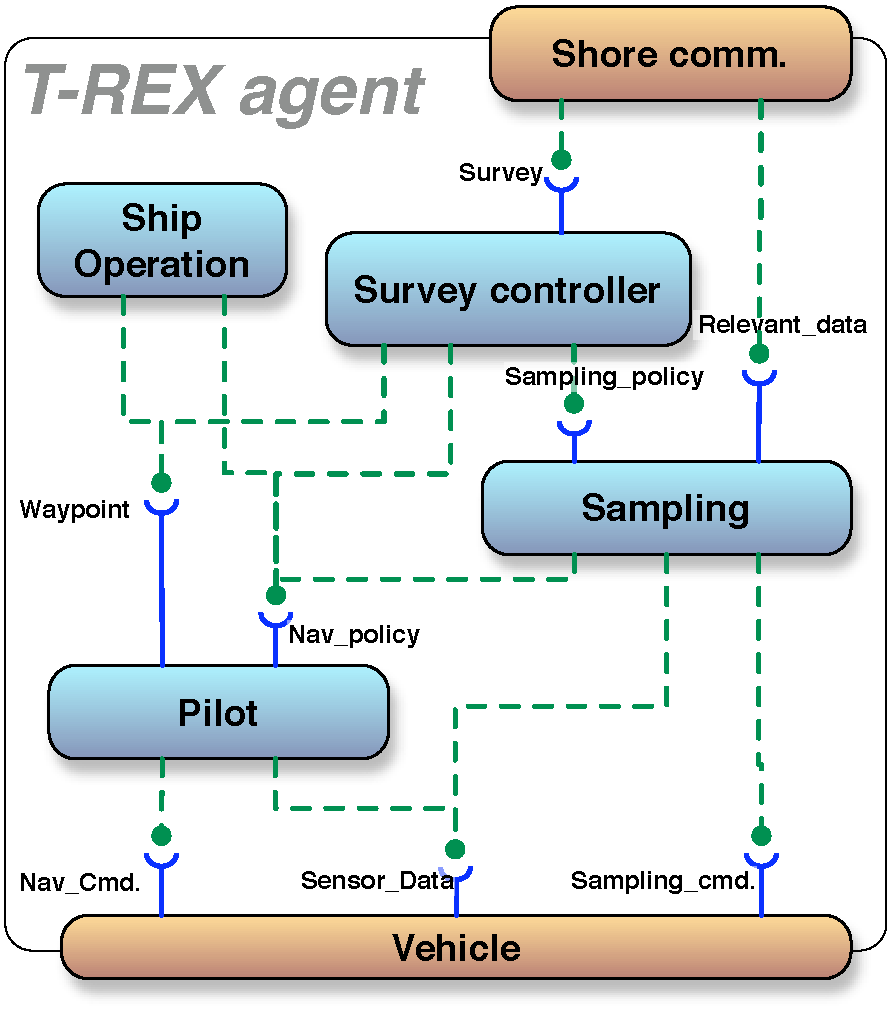
\includegraphics[scale=0.45]{figs/AUV-agent.pdf}
  \label{fig:agent}
  }
  \qquad
  \subfloat[\small State information flow between the \texttt{Pilot}
  and the \texttt{Vehicle} reactors in an \rx instance.  Observations
  transit as a bottom-up flow and apply to the execution frontier
  $\tau$.  Goal information flow from the top to the bottom and
  relates to desired future values of state variables.]{
    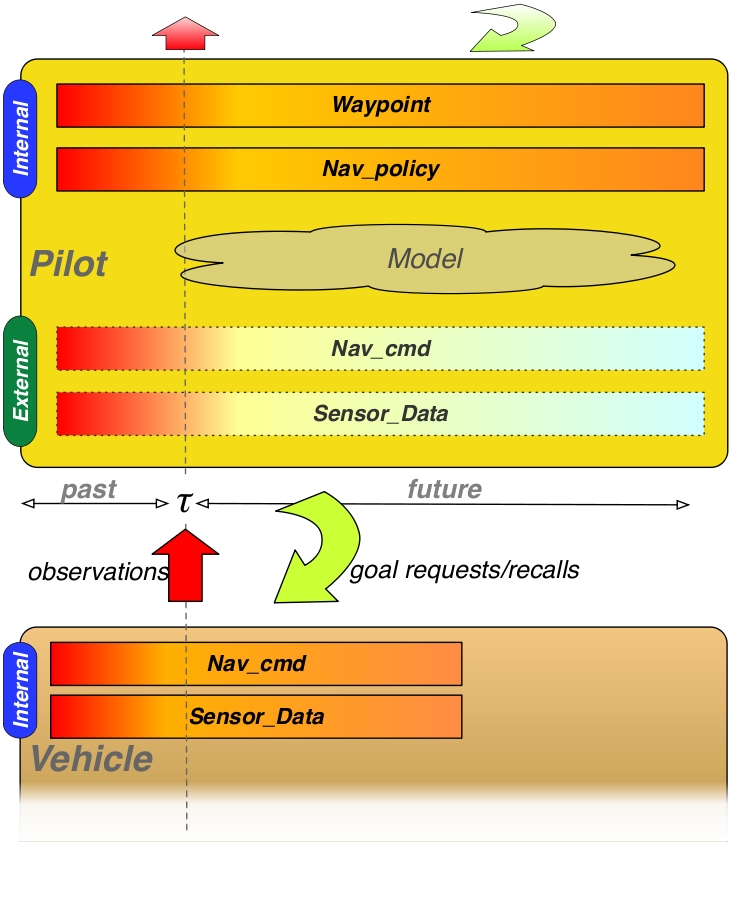
\includegraphics[width=0.4\columnwidth]{figs/TREX_flow}
    \label{fig:trex:flow}
  }
\caption{\small \rx reactors and shared state variables.}
\end{figure}

Consider for example the \rx agent instance we use on our AUV as shown
in Fig. \ref{fig:agent}. In this instance all the reactors (symbolized
by colored boxes) % do not have an explicit connection from one to
% another but instead
rely on a publish/subscribe model on shared state variables. For
instance the \textsf{Pilot} reactor needs the {\em externally} managed
state information from \textsf{Sensor\_Data} and \textsf{Nav\_cmd}
state variables in order to maintain the \emph{internal} state
variables \textsf{Waypoint} and \textsf{Nav\_policy}. This relation
applies in two ways:

\begin{itemize}

\item In order to identify its current {\em internal} state values the
  \textsf{Pilot} needs to know the current {\em external} state
  information it relies on. This information is provided in turn by
  the reactors that define these timelines as {\em internal}. In this
  specific case, the current \texttt{Waypoint} where the vehicle is
  heading can be evaluated based on the \texttt{Nav\_cmd} executed
  along with useful \texttt{Sensor\_Data}, both being provided by the
  \texttt{Vehicle} reactor.

\item The future objectives a reactor has on \textsf{Internal} state
  will likely imply sub-objectives to be reported to the owner of its
  {\em external} state variables depending on their current
  values. Should the \textsf{Pilot} want to visit a specific
  \textsf{Waypoint} -- given its current position as provided by
  \textsf{Sensor\_Data}, it can identify a sequence of
  \textsf{Nav\_cmd} states that should eventually help it reach this
  location. %\comment{this explanation could do with a figure which I
    %believe we have used previously}

\end{itemize}

Given the above example, \rx abstracts reactor interaction by
constraining them to state variables. Each reactor is therefore
agnostic where its {\em external} state information is managed as long
as this information is available and properly maintained for managing
{\em internal} state information. This {\em internal} state in turn
may be used by other reactors. Such a formalism also constrains
reactor interaction to state information exchange which comes in two
forms as illustrated in Fig. \ref{fig:trex:flow}:

\begin{itemize}

\item {\em Observation on current state values}: This information
  propagates \emph{up} in the reactor dependency graph at the
  synchronization phase and occurs at the beginning of every
  tick. During this phase the agent provides updates to each reactor
  on their {\em external} state variables for this tick so they can
  compute their {\em internal} state variable values for this same
  tick. By doing so we propagate a consistent view of that state of
  the world throughout all the reactors as time
  advances. 

\item {\em Goal request on future state}: This information propagates
  \emph{down} in the reactor dependency graph. In order to satisfy own
  {\em internal} objectives, a reactor may have a plan that relies on
  future values of one of its {\em external} state. When such a plan
  is identified the agent ensures that this part of the plan is
  provided as a goal to the owner of the given {\em external} state
  variable(s). 

\end{itemize}

The choice of representation of state variables, observations and
goals is directly derived from \eu timelines and tokens.  While such a
rich representation allows exchange of state information in a formal
yet flexible manner, its translation into planning frameworks that
have an explicit representation of time (such as but not limited to
\eue) is often trivial.

\subsection{The Execution Cycle}
\label{sec:arch:exec}

The overall execution cycle of the agent is also abstracted out as a
continuous planning/deliberation cycle between all reactors. At the
agent interface level, each reactor provides only two abstract calls
that conceptualize execution:

\begin{itemize}

\item \texttt{synchronize} takes the last set of {\em external}
  observations as an argument and returns the {\em internal}
  observations for a reactor or a failure report.

\item \texttt{step} that accepts new goals requested (if any) on the
  {\em internal} timeline of a reactor and will execute one step of
  deliberation. In the context of \eu for example, one deliberation
  step corresponds to a single flaw resolution (Section
  \ref{sec:europa:arch}) while ensuring that the resulting plan is not
  inconsistent. Backtracking is included in the step should it be such
  a case.  The returned value by the \texttt{step} function is a
  boolean which indicates whether the reactor needs an extra step to
  deliberate or if this last step resulted in a complete plan within
  the reactor's look-ahead. The part of the plan that covers the
  reactor's {\em external} timelines is provided to be dispatched as a
  goal.

\end{itemize}

Both these functions have different scope and temporal constraints.
The \texttt{synchronize} call is considered as atomic and will focus
only on state inference for the current tick by identifying the
current value of {\em internal} state variables from the latest
updates on {\em external} state variables. This process propagates up
in the reactor dependency graph at every tick to ensure that all
reactors are aware of the current state of the world. \texttt{step}
relates to a single decision step of the planning process focused on
the future evolution of state variables; it can take multiple steps
spanning multiple ticks for a reactor to produce a plan that is both
complete and valid. How the reactor identifies that its plan is
complete and valid is its responsibility and depends on the way each
reactor resolves its plan at each {\em step}. The general idea is that
the reactor is able to find a valid strategy in order to satisfy as
many of its {\em internal} goals as possible. For \eue, this means
that the solver is unable to identify any further flaws to be resolved
in the plan.

When such plan is identified, its {\em external} timeline(s) are then
dispatched to the corresponding reactors which own these times and
which in turn can start their own deliberation \texttt{step}s to
satisfy these new objectives. Consequently execution occurs as these
goals and plans propagate down in the reactor hierarchy until they
eventually become goals for the lowest level reactor which -- instead
of deliberating -- may just transform this goal into a command for
execution in hardware.

\label{sec:delib-exec-as}
\begin{figure}[!htbp]
  \centering
  \vskip-1pc
  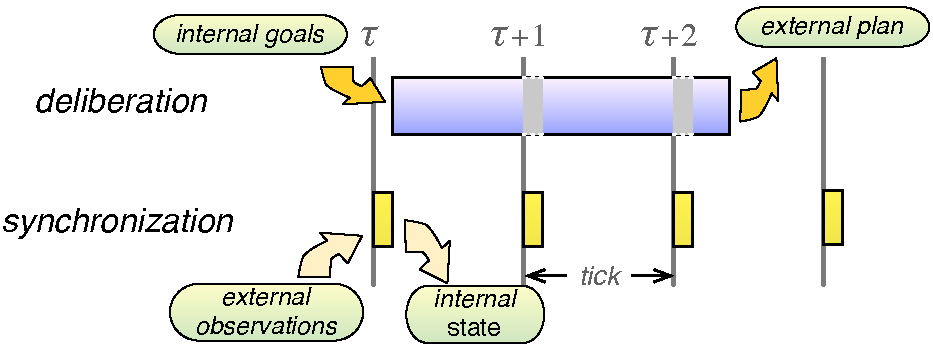
\includegraphics[width=0.55\columnwidth]{figs/tick-cycle}
  \caption{\small \rx reactor execution cycle: {\em Deliberation} is
    interrupted by {\em synchronization} at the beginning of every
    {\em tick} allowing integration of state information.}
  \label{fig:tick-exec}
  \vskip-0.8pc
\end{figure}

The manner in which the agent interleaves planning \texttt{step}s and
synchronization for a single reactor is illustrated in
Fig.~\ref{fig:tick-exec}. Synchronization occurs at every tick while
interrupting planning; this allows a reactor to identify its current
state that can propagate through the reactor hierarchy in order to
ensure a consistent view of the state of the world between all the
reactors.
% This view of a reactor has two parallel tasks allowing for long
% planning deliberation while ensuring that the state evolution
% propagates through the agent as time advance.
These intertwined tasks together provide two natural information flows
(bottom-up for state estimation and top-down for plan projection) that
we expect to see in a control loop. As they are both inference-based
processes it is natural to implement a reactor based on generic
automated planning. For example in Fig. \ref{fig:agent}, apart from
\textsf{Shore comm.} and \textsf{Vehicle} acting as interfaces, every
other reactor (in blue) is a different instance of an \eu reactor
differentiated only by their model and \eu solver configurations.

\subsubsection{Handling Failure in \rx}
\label{sec:rx-reactor-failure}

The critical task of a \rx reactor is to successfully identify its
state through synchronization as the execution frontier advances. When
a reactor fails to integrate its {\em external} state update and/or
identify its {\em internal} state at any tick, it implies that it is
unable to explain the state of the world.  This in turn implies that
any state information from this reactor is suspect, resulting in the
exclusion of this reactor from the execution cycle and consequent
destruction. As the agent destroys the faulty reactor, a special
observation, \texttt{Failed}, is produced on all {\em internal}
timelines. Reactors which declare these very state variables as {\em
  external}, are informed of the failure of this timeline.  All goals
exchanged between reactors are considered \emph{rejectable} by the
reactor that manages them. As a result in such a situation, the
failure to find a plan for these goals, is \emph{not} considered a
critical failure of the reactor. It will only result \kcomment{in}
these goals being ignored until newer goals are received.

Take for example our AUV agent from Fig. \ref{fig:agent}, and assume
that the \texttt{Sampling} reactor failed to synchronize. In such a
case this reactor is destroyed and both \texttt{Sampling\_policy} and
\texttt{Relevant\_data} timelines generate the \texttt{Failed}
observation as illustrated in Fig. \ref{fig:fail0}.  The
\texttt{Survey controller} will receive this \texttt{Failed}
observation on its {\em external} \texttt{Sampling\_policy} timeline
which indicates that this state variable is no longer managed by its
owner reactor. This leads to two potential outcomes based on how the
reactor is implemented:

\begin{enumerate}

\item The \texttt{Survey controller} model allows it to integrate the
  \texttt{Failed} observation. For example it can identify that,
  subsequent use of the water sampler is no longer possible.  The \rx
  agent can continue to navigate since \texttt{Pilot} is still
  available. In such a case the agent structure remains as in
  Fig. \ref{fig:fail0} with no consequent impact.

\item The \texttt{Survey controller} model is unable to handle this
  unexpected failure resulting in its failure to synchronize. This
  results in the \texttt{Survey controller} also failing, with
  subsequent destruction and flagging via the \texttt{Failed}
  observation on its \texttt{survey} timeline as shown in
  Fig. \ref{fig:fail1}.

\end{enumerate}

\begin{figure}[b]
  \centering
  \subfloat[\small When the \texttt{Sampling} reactor fails to
  synchronize, it is removed from the reactor dependency graph along
  with all its {\em internal} timelines while generating a \texttt{Failed} observation]{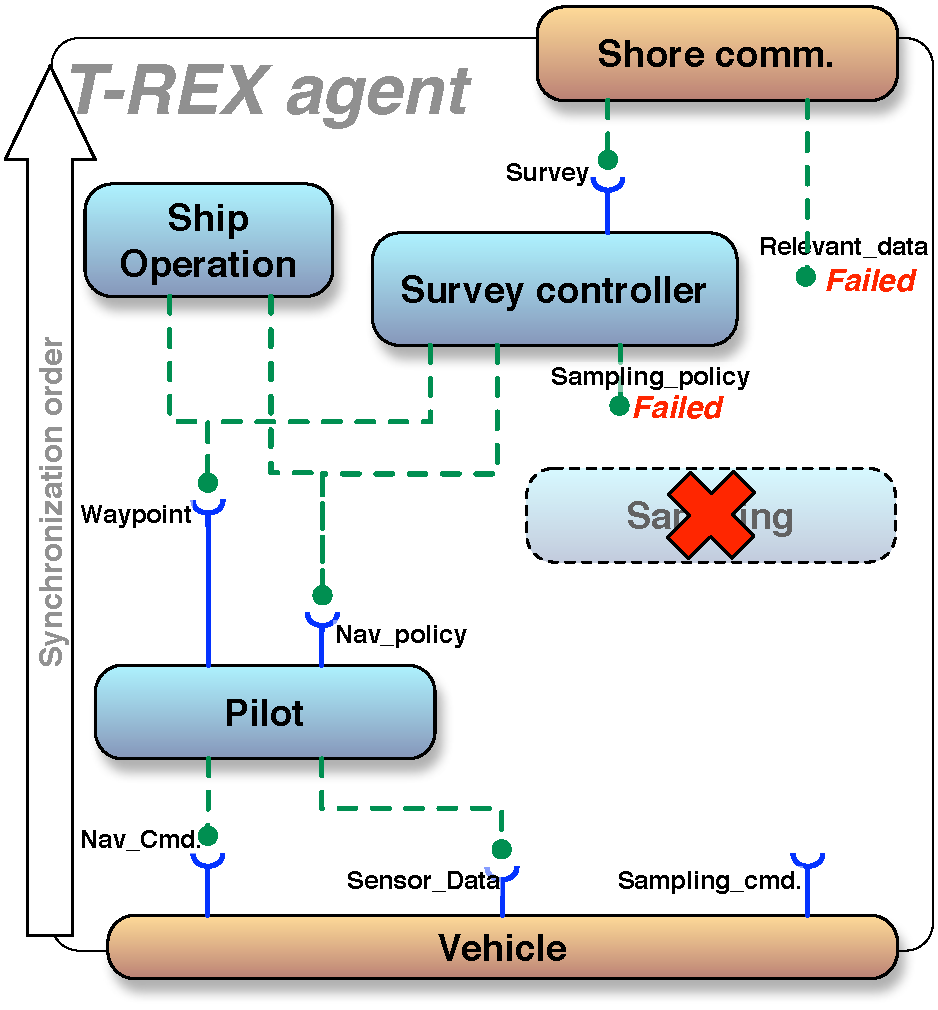
\includegraphics[width=0.35\columnwidth]{figs/AUV-fail0.pdf}
  \label{fig:fail0}}
  \qquad
  \subfloat[\small In the worst case this \texttt{Failed} observation may imply
  other reactors that depend on the \texttt{Sampling} reactor might fail to
  synchronize leading to a bottom-up destruction of ``faulty'' reactors.]{
    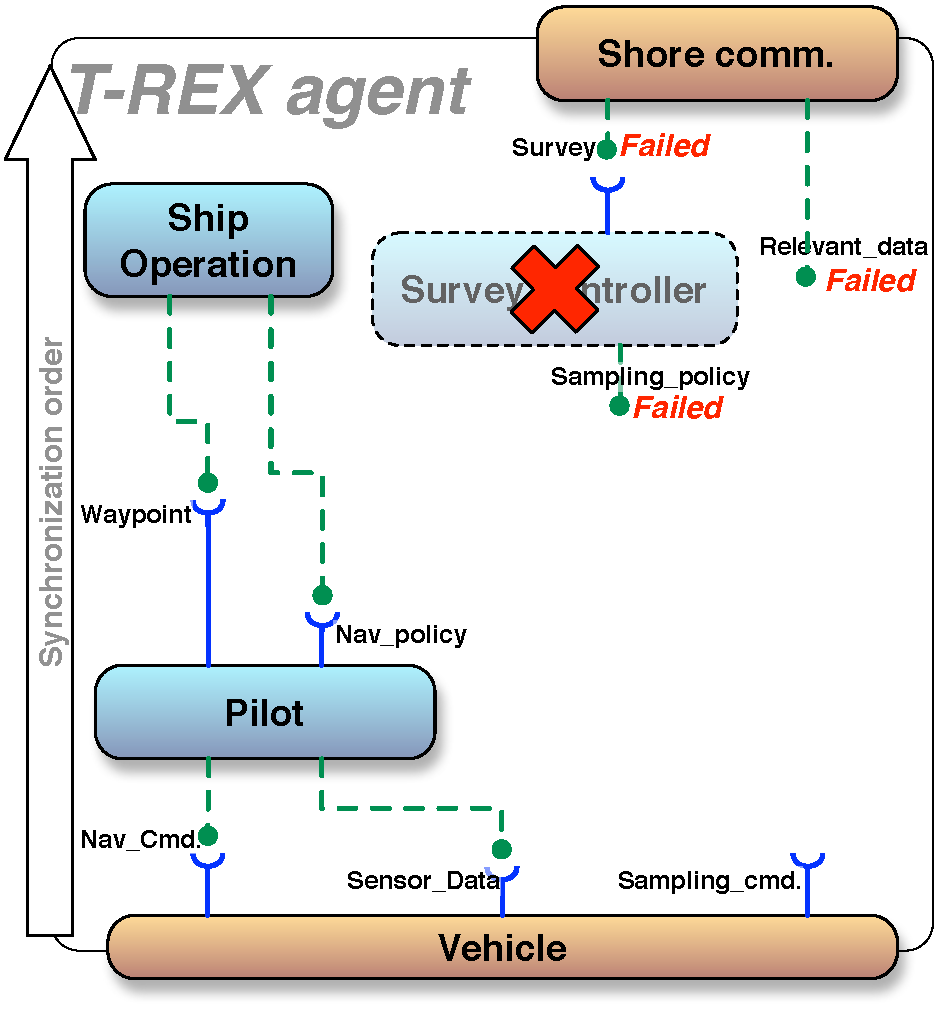
\includegraphics[width=0.35\columnwidth]{figs/AUV-fail1}\label{fig:fail1}}
  \caption{\small Impact of the \texttt{Sampling} reactor failure in
    the AUV agent \kcomment{from} Fig. \ref{fig:agent}}
\end{figure}

Even in the worst of the two cases presented above, we note that a
reactor failure only propagates \emph{up} in the reactor dependency
graph.  In our example, even if all the reactors that depend on
\texttt{Sampling} are entrained by its failure, \rx continues to keep
the reactors \texttt{Vehicle}, \texttt{Pilot} and \texttt{Ship
  operation} intact.  This ensures maintenance of vehicle control via
the \texttt{Pilot}, in addition to an abstract commanding mode for
safe operation via the \texttt{Ship operation} reactor, illustrating
how \rx can handle system degradation despite the failure of one or
more reactors, and doing so gracefully. 

Consequently, by ensuring that lower level reactors closest to the
platform hardware are robustly designed, the \rx framework ensures
that system designers can focus their attention on critical components
while factoring in deliberative control of their platforms.

\subsection{The  Deliberative Reactor}
\label{sec:arch:europa}

Within \rxe, an instance of an \eu reactor comes with the sole purpose
to deliberate. A typical design of such a reactor takes its cues from
\texttt{IDEA} \cite{mus02, mus06} where both planning and execution
are based on a single unified model within a rich representation that
provides support for temporal inference. In \rxe, the execution cycle
consists of two deliberation processes which are implemented as two
separate \eu solvers modifying the \emph{same} plan database.

\begin{enumerate}

\item The \emph{synchronization solver} is a specialized \eu solver
  that integrates new information in the plan. This signifies the
  evolution of \emph{external} timelines and ensures that the reactor
  propagates these to identify current reactor state as well as to
  inform other reactors of any state change on its \emph{internal}
  timelines. This solver is summoned at the beginning of every single
  tick.

\item The \emph{deliberation solver} manages the deliberation process
  of the reactor. It does so either to produce a new plan, to alter
  its current plan as new goals are provided or when the
  synchronization solver identifies a conflict between current state
  and expectations from a previously generated plan. This process can
  span multiple ticks and can therefore be interrupted by the
  synchronization solver.

\end{enumerate}

While the two processes are separate, they share the same plan
internal to a reactor; consequently at every synchronization cycle the
planning process is informed of the new world state and its impact on
the plan. Conversely, when synchronization occurs after deliberation
stops, its starting point is the last partial plan resulting from
deliberation. This gives an initial frame to the problem that helps to
target the synchronization problem by ensuring that the new {\em
  external} state updates are compatible with this plan. If so,
synchronization propagates these events in the plan and can use it as
an aid in resolving its {\em current state flaw}. It does so by using
the plan information on the expected {\em internal} state evolution
near the execution frontier.

If they are not compatible, then {\em synchronization} identifies a
plan inconsistency. This results in the retraction of decisions made
during previous {\em deliberation} steps.  Such a relaxation can be
viewed as a backtracking allowing the reactor to identify that its
current plan has failed to execute triggering further deliberations
steps to find an alternate strategy.

Finally, when the deliberation process has identified a complete
solution for its current {\em internal} goals, a part of its plan that
applies to its {\em external} timelines is sent as a request to \rx to
handle their dispatch to corresponding reactors.  Synchronization
eventually receives {\em external } observations that confirms plan
execution, in turn recording execution progress by having the part of
the plan observed restricted to observation start times.

Synchronization offers an important challenge for embedding planning
in a situated agent, typically an assumption to restrict the problem
to ``offline planning'' defined in \cite{ghallab04}:

{\scriptsize
  \begin{quote}
    The planner is not concerned with any change that may occur in
    $\Sigma$ \footnote{The world modeled by the plan domain.} while it
    is planning; it plans for the given initial and goal states
    regardless of the current dynamics, if any.
\end{quote}}

This assumption, while helpful to reduce the scope and complexity of
the planning problem, becomes problematic for planning within a highly
dynamic environment. In a typical robot this implies that the only
point where the planner can be informed about the current world state
is prior to the commencement of a planning cycle, by providing the
planner an initial state and current objectives. During the planning,
it is assumed that the agent can maintain the world as perceived by
the planner. \cite{lemai04, lemai-chenevier2004} attempts to reduce
the impact of planning by allowing local plan repair in the existing
plan. In the eventuality that such repair is not feasible they require
that their robot comes to a stop until (re-)planning is complete.  

This assumption is problematic for situated agents in general and as
Fig. \ref{fig:tick-exec} shows, for \rxe. Synchronization that tracks
state evolution can occur several times during reactor
deliberation. By making synchronization and deliberation share the
same plan we provide a solution that relaxes this static world
assumption. \texttt{IDEA} uses the same principle with all solvers in
an agent sharing the same plan for communicating environmental change
\cite{Dias:2003ua, mus06}. Specifically their {\em Reactive planner}
-- similar to our {\em synchronization} solver -- was often the solver
targeting the change at the execution frontier. 
% Although, none of the papers we found were detailing how this was
% handled in the architecture.
\cite{Dias:2003ua} states:

{\scriptsize
  \begin{quote}
  [\textellipsis] as long as the planning horizon over which the
  deliberative planner is working never intersects the current
  execution time, deliberative planning can operate in parallel with
  reactive execution and does not affect the reactivity of the agent. 
\end{quote}}

This suggests a deliberate non overlap between \kcomment{the} {\em
  reactive planner} and {\em deliberative planners} horizons. In \rxe,
and more specifically in our \eu reactor the planning horizon of {\em
  synchronization} -- limited to the current tick -- is a subset of
the planning horizon of the deliberation steps -- starting at the
current tick and with an extent based on latency $\lambda$ and
look-ahead $\pi$ of the reactor. In this manner we avoid creating a
conflict between the deliberation and synchronization by controlling
the scheduling of these two process\kcomment{es} by the \rx agent.

In the following sections we show how synchronization and deliberation
are implemented independently to show how their interaction through
the plan helps relax this assumption. It does so by integrating
planning in the reactor execution cycle even while allowing for more
informed deliberation.

\subsubsection{Synchronization and Identifying Internal State}
\label{sec:arch:synch}

We first show how a reactor can track and identify its state in the
context where it does not have any compelling need to deliberate. In
doing so we assume that we have a reactor that has no future
goal. Under such a condition, \rx requires each reactor to produce at
every tick its {\em internal} state. For those reactors not owning
{\em internal} timelines, \rx makes sure that {\em external}
observations are taken into account for every tick as shown in
\cite{py10}. Such a requirement is enforced to ensure that all
reactors share a consistent view of the world with advancing time.

{\em External} state updates are managed by introducing these
observations in the plan structure as facts and ensuring that they
remain compatible with the current plan maintained by the reactor. The
challenging part of synchronization is to decide the {\em internal}
state values for the current tick. In the Shopping example for example,
we have the following code snippet which helps identify when we can
\texttt{Buy} a product:

\begin{verbatim}
Agent::Buy {
  eq(duration, 10);
  // [...]
  contained_by(condition object.location.At currLocation);
  // [...]
}
\end{verbatim}

If \texttt{object.location\kcomment{.At}} is {\em external} and \texttt{Agent} is an
{\em internal} timeline, a robot may encounter the situation where it
is at the location where it can buy one (possibly among others)
product. This results in a decision-making problem related to the
state value of the \texttt{Agent} timeline; the robot can either {\em
  Buy} a specific product now, wait a little longer before doing so or
just simply not buy any product at this location.

In \texttt{T-REX}'s \eu reactor this decision-making requirement is a
new type of flaw which requires identification of all values of {\em
  internal} state variables for the current tick. This flaw can be
defined as:

\begin{definition}
  \label{def:csf}
  A {\em current state flaw} indicates that a reactor's {\em internal}
  timeline does not provide a fully defined state value for the
  execution frontier $\tau$. Such a flaw can be the result of either:

  \begin{itemize}
  \item The absence of a token in this timeline which overlaps the
    execution frontier $\tau$.
  \item An open decision between terminating the last token for this
    timeline or extending its end in the future.
  \end{itemize}

\end{definition} 

\begin{figure}[!htbp]
  \centering
  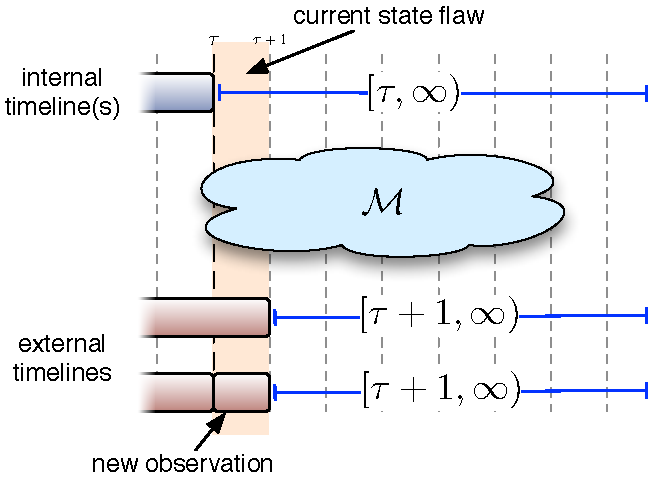
\includegraphics[width=0.5\columnwidth]{figs/synch-relation}
  \caption{\small Illustration of synchronization flaws in a
    reactor. The reactor receives new observations when they are
    produced by the owner(s) of its internal timelines. The open
    ``holes'' after the last token of each timeline represents the
    domain of all possible values for the end of this token. At every
    tick $\tau$ the reactor needs to integrate the {\em External}
    state information it received and -- based on its model
    $\mathcal{M}$ -- resolve its {\em Internal} state that will then
    be provided by the agent to other reactors using these state
    variables.}
  \label{fig:synch:flaw}
\end{figure}


The key idea is to ensure that at any single tick the {\em
  synchronization} solver will identify all the {\em internal}
timelines for which the current state value is yet to be
identified. We handle their resolution based on the following
proposition:

\begin{proposition}
  \label{prop:csf:resolve}
  A {\em current state flaw} can be resolved using one of the
  following choices which are evaluated in order:

  \begin{enumerate}

  \item Extend the previous state value to end after the execution
    frontier (\ie restrict its end time to $[\tau+1, \infty)$).

  \item Start the next active token in the timeline by restricting its
    start time to the single value $\tau$

  \item Create and insert a new token in this timeline that will start
    at the current tick $\tau$ and attempt this for each possible
    token type for this timeline if necessary.

\end{enumerate}
\end{proposition}

Intuitively the first choice enforces an \emph{inertial value
  assumption} where the reactor will tend to maintain its current
state as long as the model and external observations allow for it. The
second choice favors the advance of the reactor's current plan if any;
this directs the {\em synchronization} decision toward assuming that
its current plan is properly executed. Finally if none of these two
choices provides a valid solution -- \ie lead to an inconsistant state
-- the reactor tries all the possible state values remaining for the
timeline until it finds one that brings plan consistency.

% allows it to identify its state as required by \rx architecture.

% The flaw forces the reactor to identify its internal state for the
% current tick. By using this flaw one can describe the synchronization
% process as:

The synchronization process in turn can be described as:

\begin{enumerate}

\item Integrate the external state as provided by the owner of each
  external timeline into the plan database. 
  \begin{itemize}
  \item New observations are integrated by creating the
    corresponding token as a fact in the plan database
  \item If no observations have been received at this tick the last
    observation token restrict its \texttt{end} domaine to the
    interval $[\tau+1, +\infty)$
  \end{itemize}

\item Propagate this information in the plan database using model
  $\mathcal{M}$ of this reactor.

\item Resolve the current state value of each internal timelines based
  on Proposition \ref{prop:csf:resolve}.

\end{enumerate}

% \begin{enumerate}
% \item Integrate the external state as provided by the owner of each
%   external timeline into the plan database.
% \item Propagate this information in the plan database following the
%   model $\mathcal{M}$ of this reactor.
% \end{enumerate}

%%%% Extra paragraph:  targeted to a more AI centric audience
% The step 1 translates new {\em external} observations received from
% \rx into europa tokens with a start time restricted to $\tau$ or, for
% the timelines that did not receive a new observation,  restrict the
% previous token end time to the interval $[\tau+1, \infty)$. All of
% these tokens are produced as facts and consequently cannot be 
% excluded from the plan. They are also maintained by the reactors as
% observation tokens which will allow to avoid to mistakenly remove 
% them when one of the two reactor solvers attempt to relax former
% decisions made.\comment{This relaxation is developed on the last 
%   subsection further in depth}
%%%%

Steps $2$ \& $3$ above are handled by the \eu solver from Algorithm
\ref{alg:europa:solve} which ensures that the {\em current state
  flaws} are selected last so as to follow the sequence given above.

As {\em synchronization} focuses on the execution frontier it also
filters out all flaws that are outside of the current tick's scope.
If the flaw correlates to a token that is {\em necessarily} ending
before $\tau$ or starting after $\tau+1$ then the solver ignores
it. Such a strategy helps to reduce the scope of synchronization
exclusively to the current state of the reactor and in turn reduces
the search space for the {\em synchronization} solver.  To do so we
need to assume that the current state value of an {\em internal}
timeline does not depend on the future or more accurately that any
choice made during this {\em synchronization} will not lead to a
future inconsistency.  Such an assumption impacts the set of possible
domains the reactor can support while remaining complete. Take for
example this rule from our \texttt{Shopping} model:

\begin{verbatim}
 1 Agent::Go {
 2   met_by(condition object.location.At origin);
 3   eq(from, origin.loc);
 4
 5   equals(effect object.location.Going going);
 6   eq(going.from, from);
 7   eq(going.to, to);
 8   
 9   meets(effect object.location.At destination);
10   eq(to, destination.loc);
11 }
\end{verbatim}

While this model is perfectly acceptable for planning it becomes
problematic when execution is taken into account especially since it
puts a strong emphasis between an evolving plan and an unknown future;
\texttt{Going} to a location and the {\em expected} future outcome of
ending at this location, ties it strongly to the constraint in line
$5$ above. For instance, assume that the \texttt{Agent.location} is
{\em external} to the reactor which receives the observation
\texttt{Going(Home,SuperMarket)} which synchronization has resolved by
producing the observation \texttt{Go(Home, SuperMarket)} in the
\texttt{Agent} timeline. This would imply that the only possible
outcome on the \texttt{Agent.location} timeline, is to be
\texttt{At(SuperMarket)} in the directly foreseeable future. 

In the real world the fact that the robot is \texttt{Going} to a
certain location does not necessarily imply that it will succeed in
ending up there. Due to an exogenous event, for example, the road to
the \texttt{SuperMarket} could be closed, which could result in an
alternate observation that the robot is \texttt{At(7th st. \& Main)}
contradicting the existing plan. Further, it is important to
understand the temporal direction of the \emph{causal link} that is
triggering the inconsistency. At the time the robot observes the
contradiction of the \texttt{At} predicate, the rule that generated
this conflict is connected to past observations \texttt{Going} and
\texttt{Go}. These cannot be retracted easily without a potential
impact to the plan implying in terms of a cost in back-propagation.

More generally tying a token to future outcomes in a model that is
meant to be confronted by execution is problematic. It might be valid
if one can guarantee that an outcome is predisposed to occur (for
example the reactor managing the \texttt{Agent.location} timeline
guarantees that the outcome of the \texttt{Going} will {\em always}
result on ending at the \kcomment{target} location). However, given
the very nature of the planning problem and the ability to search
outcomes and to replan, the model should be written so that a future
projection can be manipulated.

One could therefore alter this part of the model to give the reactor
more flexibility as follows:

% \begin{minipage}[t]{\textwidth}
% \begin{figure}
\begin{verbatim}
 1 Agent::Go {
 2   met_by(condition object.location.At origin);
 3   eq(from, origin.loc);
 4
 5   contains(effect object.location.Going going);
 6   eq(going.from, from);
 7   eq(going.to, to);
 8   
 9   meets(effect object.location.At destination);
10   eq(to, destination.loc);
11   going meets destination;
12 }
\end{verbatim}
% \label{lab:model:shopping}
% \caption{\small Model fragment to enforce a \texttt{Going} end condition}
% \end{figure}
% \end{minipage}

We do so by relaxing the constraint in line $5$ from a strict
\texttt{equals} to a \texttt{contains} and to add the new constraint
at line $11$ which ensures that the last \texttt{Going} ends up in the
location the agent actually wants the robot to be at. This first level
of relaxation will therefore allow the agent to use multiple
\texttt{Going} tokens should the first one fail to reach the
objective.  

As the example above shows, synchronization involves a deliberation
process. The risk is such that the search for a solution is not a
simple sequence of decisions where the resolution can be easily
identified by the solver as any other option would lead immediately to
plan inconsistency. Since such a process is required by the \rx at
\emph{every} tick for \emph{every} reactor the model needs to be
designed carefully.

One critical aspect to take into account is that from a \rx point of
view, synchronization is the only critical task of a reactor. Such a
process is used in order for the agent to identify its current state
and maintain it consistently throughout the agent's lifetime. For a
reactor not being able to find a consistent solution during
synchronization -- implying that after evaluating all possible
solutions provided by a model it was unable to find a consistent plan
-- not only indicates that a reactor is unable to explain the state of
the world, but more importantly it may jeopardize other reactors that
rely on its {\em internal} state. For this reason a failure to
synchronize immediately results in the \rx agent killing a reactor and
notifying any reactor that depends on its {\em internal} state
variables; it does so by posting the special observation
\textsf{Failed}. This special state is a special predicate which is
acceptable for all the {\em internal} and {\em external} timelines of
\kcomment{an} \eu reactor.  By so doing we allow for graceful
degradation where other reactors can readapt their plans on receipt of
this observation.

Finally, at the engine level careful choices were made in both the
focus of the search -- limited only to tokens that can potentially
overlap the current tick -- and heuristics where the {\em current
  state flaw} is considered last during the search process. The later
limits the amount of backtracking for a solution -- or at least how
deep one needs to backtrack in a decision tree.  Similarly the
sequence in which we evaluate the possible resolution for such a flaw
-- presented in Proposition \ref{prop:csf:resolve} -- was selected
according to some simple assumptions, that any external observation
that is compatible with an existing token in the current plan reflects
the execution of the plan itself. In other words this means that our
solver always prefers to use tokens \emph{already existing} in the
plan as a way to identify current internal state. By doing so
synchronization exploits the structure of the plan produced during
previous deliberation steps.

% This implies that a deliberation steps
% have been done and did impact the plan structure and calls for a
% description on how our \eu reactor resolve such steps which we are now
% going to describe further.

\subsubsection{Deliberation: Planning for  State Evolution}
\label{sec:arch:plan}

Deliberation inside a reactor is based on \eu capabilities described
in Section \ref{sec:europa:arch}. However this deliberation comes with
some augmentation namely the reactor's deliberation latency and its
plan look-ahead both expressed in ticks and that the agent needs to
interleave deliberation with not just the synchronization but also
with deliberation of other reactors\footnote{The current
  implementation of \rx is running on a single process and it is the
  responsibility of the agent itself to emulate reactor
  multi-threading for deliberation and synchronization.}.  For this
reason while the reactor relies on the \eu solver, it slices the
execution of Algorithm \ref{alg:europa:solve} into atomic steps. This
interruption occurs around the recursive call line \ref{li:recurse}
while ensuring that the current partial plan is not inconsistant at
any single step. This is managed by allowing the call to backtrack
until a \textsf{DecisionPoInt} that is not exhausted (\ie
$decision.hasNext()$ is \texttt{true}) is found in the call stack.

A critical aspect of this deliberation step is to ensure that at the
exit of this call the $plan$ is not inconsistent. % Indeed, it is always
% possible that the next call made by the agent is for synchronization
% which could fail if the $plan$ is inconsistent before any attempt is
% made for synchronization.
If the partial plan is found to be inconsistent during a deliberation
step we either backtrack in the decision stack until a node of the
tree is found with an alternate solution or the plan is relaxed since
there is no other alternative solution. We do this by removing all
goals while keeping only recent observations. 

{\em Synchronization} and the dispatching of new {\em goals} from \rx
can occur between two steps and alter the plan. These alterations
exogenous to the deliberation process dynamically impact the set of
flaws that need to be resolved. New flaws are created when a new goal
is received from \rx and conversely the recall of an objective could
remove the corresponding flaws\footnote{However if the flaws related
  to this goal were resolved, the removal of this goal may likely
  create new flaws.}. The impact of {\em synchronization} can be more
subtle as its alteration of the plan at the execution frontier is more
drastic. We can still give a non exhaustive list of possible
alterations of the flaws directly related to {\em synchronization}:

\begin{enumerate}

\item Previous flaws directly related to the execution frontier have
  been resolved by the {\em synchronization} solver.

\item The {\em synchronization} solver may have created new flaws that
  were outside of its scope but are now part of the scope of the {\em
    deliberation} solver.

\item The last observation has proved that the current plan is invalid
  requiring the {\em synchronization} solver to relax the existing
  plan to identify its current {\em external} state. (This case is
  developed further \kcomment{in} the next section).

\end{enumerate}

\begin{figure}[!htbp]
  \centering
  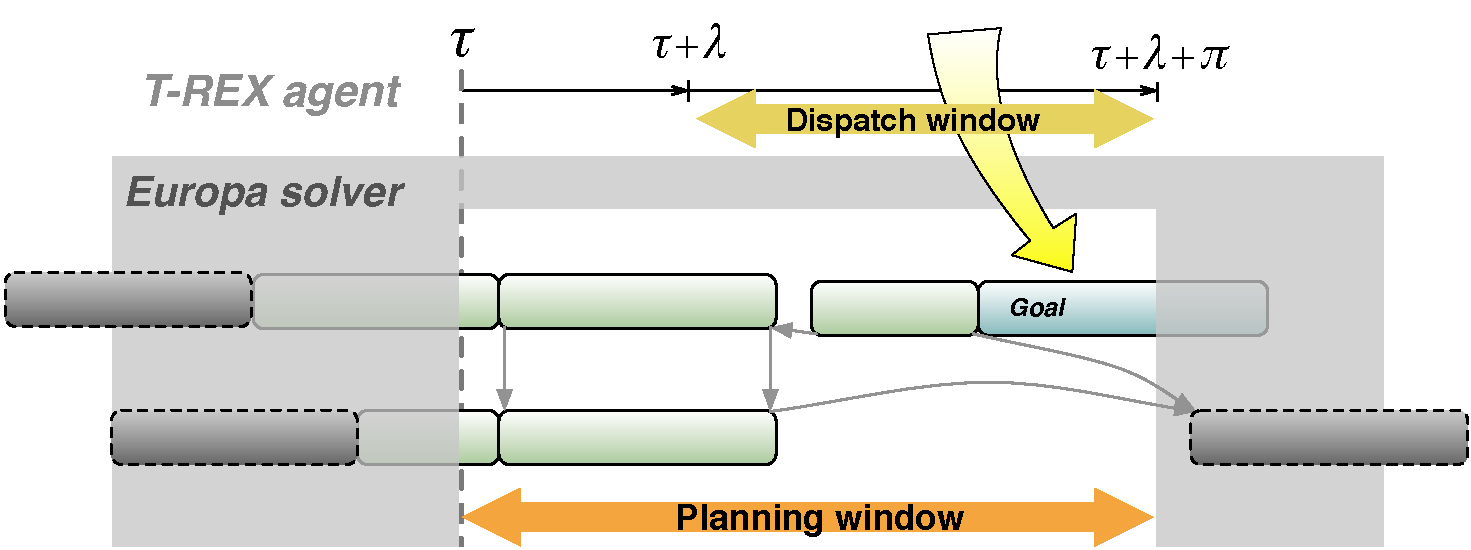
\includegraphics[width=0.65\columnwidth]{figs/plan_window}
  \caption{\small The planning window of the deliberation solver and
    its relation to the {\em dispatch window}. The dark grey tokens
    with dashed borders are excluded from deliberation as they do not
    overlap the interval $[\tau, \tau+\lambda+\pi]$. All the other
    tokens ({\color{green} green}) along with the goals received from
    the agent ({\color{blue} blue}) which can overlap this window, are
    evaluated.}
  \label{fig:plan:window}
\end{figure}

When the {\em execution frontier} advances, the reactor planning scope
moves further into the future. This is reflected by the {\em
  deliberation} solver which uses a new deliberation scope one tick
further in the future. As Fig. \ref{fig:plan:window} illustrates, such
a scope allows filtering of tokens that are either necessarily ending
before $\tau$ or necessarily starting after, focusing the planning
problem on only those tokens that are within a ``reasonable'' future.
This filtering window complements the \rx {\em dispatch window} from
Definition \ref{def:dispatch} which filters out at the agent level
those goals that are before the reactor execution latency or too far
into the future.  The planning window refines this filtering further,
as tokens can be excluded dynamically from deliberation as their
insertion in the plan and scheduling with other generated tokens can
alter their temporal scope to be outside of the planning window.  This
allows the planner to focus on its planning horizon and report
decision on flaws that are beyond this scope. As time advances, these
potential future flaws will eventually be part of the planning window
of the reactor and will be then resolved along with potentially new
goals.  This in turn, results in an apparent \emph{continuous
  planning} of the reactor. When there are no more flaws present in
the current planning scope a partial plan solution is found. This has
two effects:

\begin{enumerate}

\item This reactor does not need to deliberate until the next
  synchronization. 

\item The token on the {\em external} timelines of this partial plan
  can then be posted which eventually (at the end of the current tick
  if these goals overlap the owner reactor's planning window) will be
  dispatched as goals, in turn triggering further deliberation.

\end{enumerate}


\subsubsection{Interleaving Synchronization and Execution}
\label{sec:arch:intertwine}

A key aspect of the \rx framework is interleaved plan and
execution. Both {\em synchronization} -- keeping track of execution --
and {\em deliberation} -- dealing with reactor planning -- of one
reactor are sharing the same {\em single} plan database which 
they modify alternatively as the \rx agent schedule their execution.

As noted above, it is synchronization which drives planning, so the
co-mingling between these two processes is critical to maintaining
state within a robot especially when it is immersed in a dynamic
environment. Further, it is important that \rx maintain
% A core aspect of this reactor is that it takes advantage of the
% specific sequencing enforced by the \rx architecture along with the
% fact that only 
one $plan$ structure shared between synchronization and planning. This
allows these two processes to not only be interleaved for agent
responsiveness, but ensures a viable mechanism to communicate.

% but also impact
% each other via plan manipulation.

As noted earlier, synchronization propagates {\em
  external} observations when a new tick occurs. Earlier, we isolated
the case when a reactor has no future goal or no plan to enforce. By
doing so we were able to develop the way we augment the \eu solver to
propagate {\em external} observations to identify {\em
  internal} state. This allowed us to focus on synchronization as a
state evaluation process that can be resolved within the \eu framework
with few extensions. Similarly we presented deliberation as an
abstraction without discussing the disruptive nature of
synchronization and how it impacts the planning process. We first
analyze the case when synchronization occurs after planning has
completed (\ie the last step of deliberation results in a plan that is
considered complete for the current look-ahead). As synchronization
starts with a plan, this deliberation will not only be a model-derived
estimation uniquely based on {\em external} observations but will also
include reactor intentions specified in the available partial plan.

Consider for example the Shopping Agent model where the timeline 
\texttt{Agent.position} is {\em external} while \texttt{Agent} is
implemented a an {\em internal} timeline. As the reactor adds a goal to
\texttt{Own} milk and the current {\em external} timeline indicates
that the robot was \texttt{At(home)}, it produces a plan as shown in
Fig. \ref{fig:shop:exec0}. The {\em external} part of the plan --
namely the tokens \texttt{Going(home, superMarket)} and
\texttt{At(SuperMarket)} -- are installed as goals for the reactor
managing this state variable internally.

\begin{figure}[!b]
  \centering
  \subfloat[\small A plan produced before
  synchronization.]{\label{fig:shop:exec0}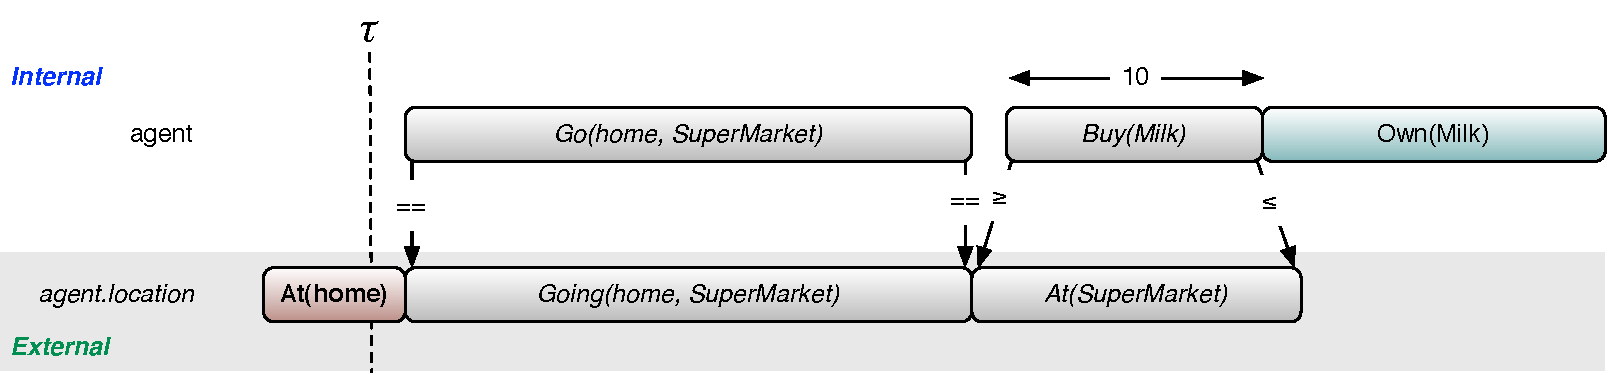
\includegraphics[width=0.7\columnwidth]{figs/shoping_exec_t0}} \\
  \subfloat[\small Result of synchronization after the {\em Going}
  observation was received by the reactor with the plan showed in
    \ref{fig:shop:exec0}.]{\label{fig:shop:exec1}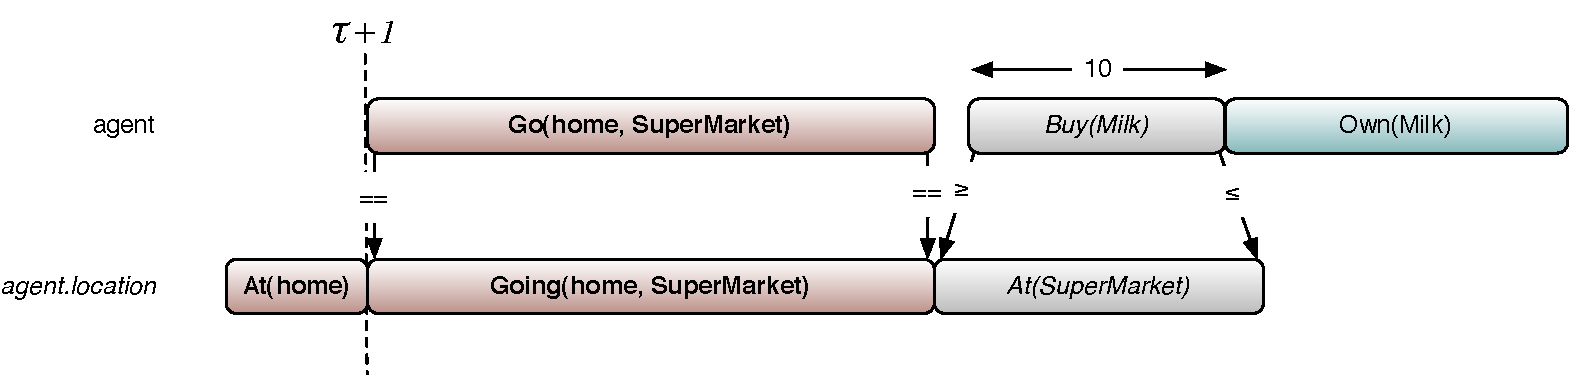
\includegraphics[width=.7\columnwidth]{figs/shoping_exec_t1}}
    \caption{\small The Shopping example: Tokens in {\color{red}red}
      indicate observations, tokens in {\color{blue}blue} the goal
      that this plan attempts to solve for. Arrows indicate temporal
      constraints. }
  \label{fig:shop:exec}
\end{figure}

Consider that at the next tick $\tau' = \tau+1$ the reactor managing
agent location is able to change the location state variable to
\texttt{Going}. \rx informs the reactor of this observation which is
added to the partial plan as a fact -- starting exactly at $\tau'$ and
lasting for an unknown duration which is at least one tick. As this
new observation is integrated in the plan through synchronization, the
solver can identify the similarity between this observation and the
next token in the existing plan. Instead of initiating an exhaustive
search of all possible implications, the synchronization process
starts its execution with the assumption that these new observations
are consistent with the currently maintained plan. As a consequence,
at the end of synchronization the plan depicted in Fig.
\ref{fig:shop:exec1} is likely. This is a result of propagation of
information provided by the new observation in the existing plan while
restricting the start time of \texttt{Going} and propagating temporal
constraints, making \texttt{Go} to start {\em exactly} at $\tau'$. In
doing so, the \eu solver's focus on the execution frontier ($\tau'$ in
Fig. \ref{fig:shop:exec1}) takes advantage of the existing plan to
evaluate a solution that assumes that the observation is consistent
with what was decided by the reactor.

% \begin{figure}[!htb]
%   \centering
%   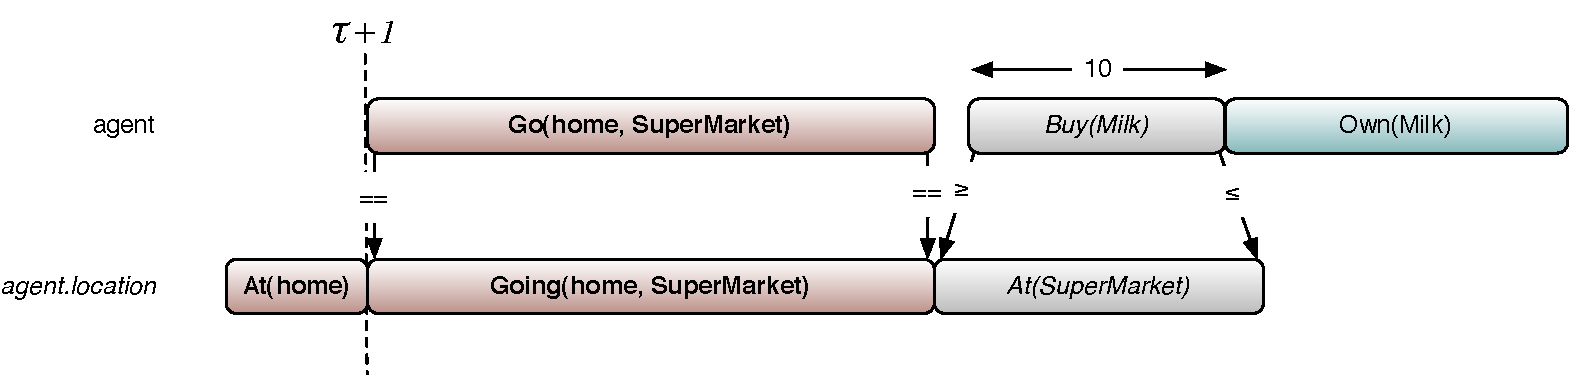
\includegraphics[width=0.7\columnwidth]{figs/shoping_exec_t1}
%   \caption{Shopping example : Result of synchronization after the {\em
%       Going} observation was received by the reactor with the plan
%     showed in Fig. \ref{fig:shop:exec0}.}
%   \label{fig:shop:exec1}
% \end{figure}

This choice is directed not only by heuristic choices made in the
solver but also enforced by the heuristic order of the decision point
resolution choices for the {\em current state flaw} shown in
Proposition \ref{prop:csf:resolve}. As noted, the first two choices
are biased towards a conservative view with respect to the existing
plan. The heuristics first attempt to extend the previous observation
for this {\em internal} timeline to avoid early commitment. If this
fails \rx attempts to start the next existing token in the plan to
advance plan execution. Both choices attempt to resolve state with the
least amount of plan perturbation by constraining further the start
and end time of existing tokens generated by previous deliberations
steps. By doing so, in a nominal situation, synchronization remains
limited to restrict time points in the plan and propagates their
impact. Most of the computational effort of creating new tokens in the
plan and scheduling them onto timelines are managed during
deliberation steps. Consequently, most of the time synchronization is
limited to very few nodes in the \eu search space often requiring no
backtracking. Fig. \ref{fig:shop:exec} shows how the existing plan can
support the synchronization process. The observation \texttt{Going}
occurring at $\tau'$ is fully compatible with the token already present
in our plan. By updating the plan and propagating equality constraints,
the resolution of the {\em current state flaw} for the {\em Agent}
timeline becomes obvious as a solution, as the token \texttt{Go} from
the plan presents itself.

Synchronization may become computationally more expensive when we need
to identify a new token to be injected into the plan (the third choice
in Proposition \ref{prop:csf:resolve}), as it needs to explore the
outcome of inserting all possible token types the timeline can accept.
This is the reason this choice is evaluated last in our flaw
resolution strategy.

% In that sense, and thanks to the careful choice on our
% synchronization heuristic we see that the plan produced during \rx
% deliberation steps helps the synchronization process to be more
% efficient.

% Should such a flaw be revealed 
% during synchronization -- such that the current state of
% an {\em internal} state variable is not fully grounded -- the
% sequencing of the choices will attempt first a conservative choice in
% maintaining previous state and only then try a more optimistic
% approach in terms of the \comment{I don't follow this last bit. Is
%   this token addition that you're talking about?} execution/advance in
% our current plan to finally attempt other choices that were not
% predicted by the model. The two first possible choices are strongly
% directed by the existing plan which helps direct the search within
% this frame. This often allow to have a synchronization that is much
% more directed and, in nominal cases such as the one we showed resolve
% the deliberation in few steps (often without any backtrack in the
% search) \comment{All this is confusing; probably reword}.

Synchronization also supports the tracking of plan execution. It does
so by specifying token parameters such as time points that are
propagated throughout the plan to identify plan validity.
%  -- as in our example -- or that it cannot be executed as it is. 
When invalid, identification occurs by synchronization failing to find
a consistent solution. For example should the \texttt{Going}
observation received be to the \texttt{hardwareStore}, this would
break the partial plan in the reactor as the robot cannot possible be
going simultaneously to two different locations; see Fig.
\ref{fig:shop:relax1}. As synchronization is not possible in such a
situation the strategy followed is to relax all decisions made by
previous plan steps. This is done by keeping all past observations in
both {\em external} and {\em internal} state variables as well as the
existing {\em internal} goals (\texttt{Own(Milk)} in this example)
received by the reactor. The resulting partial plan is shown in Fig.
\ref{fig:shop:relax2}. In this process the reactor informs the agent
that all {\em external} goals it requested for the future are no
longer valid, allowing timeline owners to divest maintaining such
goals.

\begin{figure}[!b]
  \centering
  \subfloat[Conflicting Observation]{\label{fig:shop:relax1}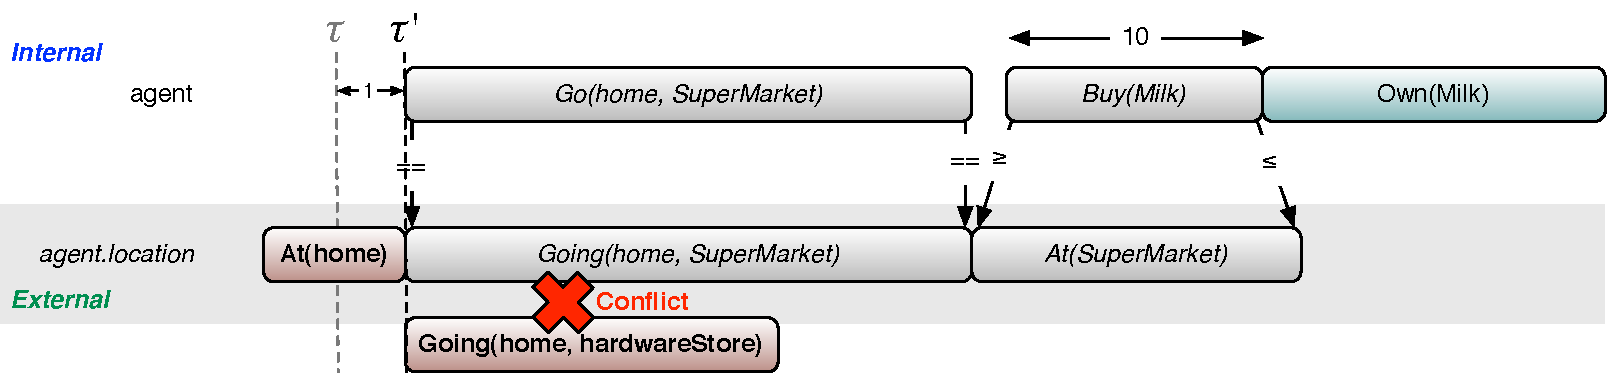
\includegraphics[width=0.7\columnwidth]{figs/shoping_exec_relax-1}}\\
  \subfloat[Relaxed Partial Plan]{\label{fig:shop:relax2}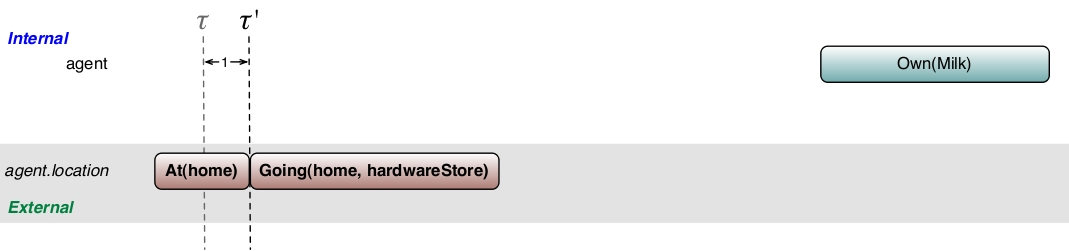
\includegraphics[width=0.7\columnwidth]{figs/shoping_exec_relax-2}}
  \caption{\small Illustration of a conflict during synchronization
    and the resulting relaxed plan for recovery.}
\end{figure}

When the plan is no longer conflicted, synchronization can resume and
find a solution as described above. Newly pending goals would be
enforced at the next \texttt{step} to resume deliberation on this
relaxed partial plan. By using synchronization the reactor is not only
able to identify that the plan is consistent but able to recover from
it by offering a new incomplete partial plan to be resolved in the
next deliberation \texttt{steps}. % This on its own offer the core
% functionality one should except to close the loop between planning and
% execution in the sense that 
Synchronization therefore, plays the role of what is typically termed
as the {\em Executive} in other architectures \cite{gat98,
  alami:1998p820, mus98, williams03, Nesnas:2003do}.

In \rx however the interaction between planning and execution does not
stop at this level. The overall scheduling of both {\em
  synchronization} and {\em planning} is such that the synchronization
can occur in between any planning step. Not only is synchronization
influenced by the outcome, but it also influences planning.
Specifically when synchronization occurs before a complete plan is
found, it will inject new facts ({\em external} observations and
resulting {\em internal} state) in the plan database available for
inference when the next planning \texttt{step} resumes. On this next
step the \eu solver used for planning will have these new facts
included in the partial plan which can introduce new flaws in the plan
while potentially having resolved previously existing flaws. The
deliberation process is therefore perturbed externally by {\em
  synchronization} and consequently fully informed of the world state
evolution as it is planning. This contrasts with other classical
approaches, which avoid perturbing the planner during its search as it
is not compatible with the ``off-line planning'' assumption, noted in
Section \ref{sec:arch:europa}.

By design choices made in the \rx framework -- both at the
architectural level and the integration of the \eu framework for
embedded deliberation -- we are able to implement a system that avoids
this critical off-line planning limitation while enforcing a formal
framework that allows for deliberation and model-based agent control.
This tight integration of planning and execution allows the system to
be more responsive to environmental change allowing informed
decision-making within a tighter reaction loop and despite reactor
latency.


% As long as one can ensure that synchronization of all
% reactors and deliberation steps can be done within a time that is
% reasonably small in comparison to the agent tick duration.



% Gives a high-level overview of T-REX, the general design principles and how
% these principles aid in software engineering. Show T-REX block diagram.



%%% Local Variables: 
%%% mode: latex
%%% TeX-master: "setobook"
%%% End: 
